\documentclass[]{article}
\usepackage{geometry}
\geometry{
	a4paper,
	total={170mm,257mm},
	left=0.75in,
	top=0.75in,
	right=0.75in,
	bottom=1in,
}
\usepackage{gensymb}
\usepackage{lipsum}
\usepackage{graphicx}
\usepackage{amsmath}
\usepackage{xcolor}
\usepackage[
  colorlinks,
  breaklinks,
  unicode
]{hyperref}
\usepackage{listings}
\newcommand\Colorhref[3][blue]{\href{#2}{\color{#1}#3}}
\title{\textbf{Beginner's guide to Basilisks}}
\author{Vatsal Sanjay\\vatsalsanjay@gmail.com}
\begin{document}
\maketitle
\begin{abstract}
This document is a review and guide to the installation and working of Basilisk \Colorhref{http://basilisk.fr/}{(link)}, written by St\'ephane Popinet and his group. These notes are for personal use only, and detailed guide could be found at \Colorhref{http://basilisk.fr/Tutorial}{$<$link$>$}.\\\par 
Regarding this file: Since basilisk is still in the early stages of development, the facts written in this document are subject to change. If you find any information here outdated or incomplete, please let me know.
\end{abstract}
\section{Installing Basilisk}
Installation is quite easy. There are two ways: Using darcs OR using tarball. I prefer the first one (darcs) because it allows to easily pull any update that occurs in Basilisk. The steps of this section are taken from \Colorhref{http://basilisk.fr/src/INSTALL}{http://basilisk.fr/src/INSTALL}. They are self-explanatory I have included them here, just for the sake of completion. 
\subsection{Installing darcs (if unavailable)}
{\color{red}vatsal@cloneMachine:$\sim\$$} sudo apt-get install darcs flex make
\subsection{Some important side packages}
{\color{red}vatsal@cloneMachine:$\sim\$$} sudo apt-get install gnuplot imagemagick libav-tools smpeg-plaympeg graphviz valgrind gifsicle
\subsection{Getting Basilisk source code}
{\color{red}vatsal@cloneMachine:$\sim\$$} darcs get http://basilisk.fr/basilisk
\begin{figure}[h]
\centering
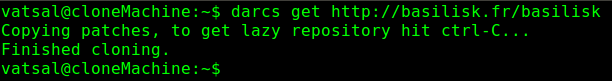
\includegraphics[width=0.75\linewidth]{Figure1}
\end{figure}
\paragraph{\textbf{Note:}} In order to pull new changes made in Basilisk, use:\\
{\color{red}vatsal@cloneMachine:$\sim\$$} cd basilisk\\
{\color{red}vatsal@cloneMachine:$\sim\$$} darcs pull\\
Then recompile.
\subsection{Compiling/recompiling Basilisk}
{\color{red}vatsal@cloneMachine:$\sim\$$} cd basilisk/src\\
{\color{red}vatsal@cloneMachine:$\sim\$$} export BASILISK=\$PWD\\
{\color{red}vatsal@cloneMachine:$\sim\$$} export PATH=\$PATH:\$PWD\\
{\color{red}vatsal@cloneMachine:$\sim\$$} ln -s config.gcc config\\
{\color{red}vatsal@cloneMachine:$\sim\$$} make -k\\
{\color{red}vatsal@cloneMachine:$\sim\$$} make

\section{Basilisk-View}
Details of bview: \Colorhref{http://basilisk.fr/src/README\#interactive-basilisk-view}{http://basilisk.fr/src/README\#interactive-basilisk-view}\\
Basilisk-view is similar to GfsView, with some minor differences:
\begin{enumerate}
\item Unlike GfsView, we cannot run bview on the fly while basilisk is running. We can, however, use it to render pictures and videos on the fly with bview. It can be used to look at the results after simulation is over, provided we have saved the intermediate files.
\item There is no program written analogous to gfs2oogl for bview. This means that we cannot interpolate the octree based data using available libraries. We could write our own code for it in future, something similar to gfs2oogl.
\item I found a working example for tecplot users \Colorhref{http://basilisk.fr/sandbox/hiroumi/tecplot/}{(here)}, but I have not tested it yet. 
\end{enumerate}
GfsView can still be used with Basilisk, provided that the code does not use \textquotedblleft mask\textquotedblright command. Mask command is used for creating solid objects and non-square (non-cubical) geometries. The precursor to using gfsview and writing \textquotedblleft.gfs\textquotedblright files, \textquotedblleft dump\textquotedblright is not compatible with \textquotedblleft mask\textquotedblright. Most likely, even bview cannot be used to look at intermediate files when \textquotedblleft mask\textquotedblright is used, but I have not changed it. For other compatibility issues, visit: \Colorhref{http://basilisk.fr/src/COMPATIBILITY}{http://basilisk.fr/src/COMPATIBILITY}.
\subsection{Installing bview}
Sources: (go in this order)
\begin{enumerate}
\item bview: \Colorhref{http://basilisk.fr/src/bview}{http://basilisk.fr/src/bview}
\item Screen rendering: \Colorhref{http://basilisk.fr/src/gl/INSTALL}{http://basilisk.fr/src/gl/INSTALL}
\item Python for bview-client: \Colorhref{http://basilisk.fr/src/bview-client.py}{http://basilisk.fr/src/bview-client.py}
\item Actual installation: \Colorhref{http://basilisk.fr/src/bview-server.c}{http://basilisk.fr/src/bview-server.c}
\end{enumerate}
\subsubsection{Dependencies}
For cluster for off-screen rendering:\\
{\color{red}vatsal@cloneMachine:$\sim\$$} sudo apt-get install libglu1-mesa-dev libosmesa6-dev\\
{\color{red}vatsal@cloneMachine:$\sim\$$} cd \$BASILISK/gl\\
{\color{red}vatsal@cloneMachine:$\sim\$$} make libglutils.a libfb\_osmesa.a\\
Another method would be to use the following (recommended for laptops), the above dependencies are recommended for clusters.\\
{\color{red}vatsal@cloneMachine:$\sim\$$} sudo apt-get install libglu1-mesa-dev libglew-dev libgl1-mesa-dev\\
{\color{red}vatsal@cloneMachine:$\sim\$$} cd \$BASILISK/gl\\
{\color{red}vatsal@cloneMachine:$\sim\$$} make libglutils.a libfb\_glx.a\\
The following is required for both the above versions:\\
{\color{red}vatsal@cloneMachine:$\sim\$$} sudo apt-get install python-pil.imagetk
\subsubsection{bview}
Add this line at the end of config.gcc, depending on the type of machine and dependency selected:\\
Osmesa (Cluster):
\begin{verbatim}
OPENGLIBS = -lfb_osmesa -lGLU -lOSMesa
\end{verbatim}
Glx (Laptop):
\begin{verbatim}
OPENGLIBS = -lfb_glx -lGLU -lGLEW -lGL -lX11
\end{verbatim}
Then do this:\\
{\color{red}vatsal@cloneMachine:$\sim\$$} cd \$BASILISK\\
{\color{red}vatsal@cloneMachine:$\sim\$$} make bview-servers\\
For a typical bview use and environment, follow the example at:\Colorhref{http://basilisk.fr/src/bview}{http://basilisk.fr/src/bview}
\section{A typical code}

\end{document}
